\chapter{مقدمه}
    \section{ پیش زمینه}
        \subsection{کشف آنزیم ها از متاژنوم ها}
            متاژنومیکس با امکان تجزیه و تحلیل مستقیم مواد ژنتیکی بازیابی شده از نمونه های محیطی، مطالعه جوامع میکروبی را متحول کرده است. برخلاف روش‌های سنتی مبتنی بر کشت، متاژنومیکس دسترسی به تنوع میکروبی گسترده‌ای را فراهم می‌کند که در شرایط آزمایشگاهی غیرقابل کشت باقی می‌ماند. این رویکرد منجر به کشف آنزیم های جدید با خواص کاتالیزوری منحصر به فرد شده است که بسیاری از آنها کاربردهای صنعتی و بیوتکنولوژیکی قابل توجهی دارند.
            در میان این آنزیم ها، زایلانازها به دلیل توانایی آنها در تجزیه زایلان، دومین پلی ساکارید فراوان در طبیعت، از اهمیت ویژه ای برخوردار هستند. زایلانازها زایلان را به قندهای ساده‌تر تجزیه می‌کنند و آنها را برای تولید سوخت زیستی، فرآوری غذا و خوراک و کاربردهای صنعتی ضروری می‌سازد. شناسایی آنزیم‌های زایلاناز جدید از متاژنوم‌ها می‌تواند منجر به بیوکاتالیست‌های کارآمدتر با پایداری، فعالیت و ویژگی سوبسترای بهتر شود.
        \subsection{اهمیت زایلانازهای میکروبی}
            زایلانازهای میکروبی نقش مهمی در صنایع مختلف دارند:
            \begin{itemize}
                \item \textbf{تولید سوخت زیستی:}زایلانازها به تجزیه زیست توده گیاهی به قندهای قابل تخمیر کمک می کنند و عملکرد بیواتانول را بهبود می بخشند.
                \item \textbf{صنعت خمیر و کاغذ:} در فرآیندهای سفید کردن سازگار با محیط زیست برای کاهش استفاده از مواد شیمیایی و بهبود کیفیت کاغذ استفاده می شود.
                \item \textbf{فرآوری غذا و خوراک:} افزایش قابلیت هضم در خوراک دام و بهبود بافت محصولات پخته شده.
                \item \textbf{کشاورزی و بیوتکنولوژی:} کمک به تخریب زیست توده گیاهی، ترویج شیوه های کشاورزی پایدار.
            \end{itemize}
            با توجه به اهمیت صنعتی آنها، کشف زایلانازهای مقاوم در برابر حرارت و مقاوم در برابر pH بسیار ارزشمند است. این خواص عملکرد آنزیم را در شرایط شدید افزایش می دهد و آنها را در فرآیندهای صنعتی موثرتر می کند.
            \begin{figure}[H]
                \centering
                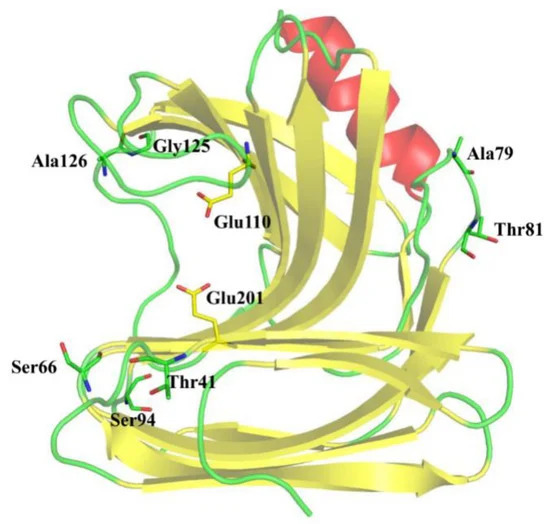
\includegraphics[width=0.8\textwidth]{images/xylanase.jpg} % Replace with your image file
                \caption{xylanase}
                \label{fig:xylanase}
            \end{figure}
        \subsection{چرا متاژنوم شکمبه؟}
            میکروبیوم شکمبه نشخوارکنندگان یک مخزن غنی از میکروارگانیسم های تجزیه کننده لیگنوسلولز است. نشخوارکنندگان برای تجزیه موثر مواد گیاهی به جوامع میکروبی خود متکی هستند و شکمبه را به محیطی ایده آل برای جستجوی آنزیم های زایلاناز جدید با فعالیت قوی تبدیل می کند. با تجزیه و تحلیل توالی‌های متاژنومی مشتق شده از شکمبه، محققان می‌توانند زایلانازهای جدیدی را کشف کنند که برای عملکرد تحت شرایط فیزیولوژیکی طبیعی تکامل یافته‌اند و اغلب پایداری در دمای بالا و انعطاف‌پذیری در محیط‌های 
            pH 
            اسیدی یا قلیایی از خود نشان می‌دهند.

            هدف این پروژه شناسایی و مشخص کردن ژن‌های کدکننده زایلاناز از متاژنوم شکمبه، استفاده از ابزارهای بیوانفورماتیک برای شناسایی توالی، خوشه‌بندی و مدل‌سازی منطقه حفاظت‌شده است. نتایج ممکن است به کشف زایلانازهای مرتبط صنعتی جدید کمک کند و درک ما را از تخریب لیگنوسلولز میکروبی در اکوسیستم شکمبه افزایش دهد.

    \section{اهداف}
        هدف اصلی این مطالعه شناسایی و شناسایی ژن‌های کدکننده زایلاناز از متاژنوم شکمبه نشخوارکنندگان، با استفاده از روش‌های بیوانفورماتیک برای شناسایی، خوشه‌بندی و تجزیه و تحلیل توالی‌های زایلاناز پایدار حرارتی بالقوه است. با توجه به اهمیت صنعتی زایلانازها در سوخت‌های زیستی، غذا، خوراک و پردازش کاغذ، هدف این مطالعه کشف زایلانازهای جدیدی است که ممکن است کارایی و پایداری را در شرایط شدید ارائه دهند.

        برای دستیابی به این هدف، پروژه در سه هدف اصلی ساختار یافته است:
        \begin{enumerate}
            \item شناسایی توالی های بالقوه زایلاناز
                \begin{itemize}
                    \item جستجوهای مبتنی بر شباهت را با استفاده از ابزارهایی مانند 
                    BLAST، DIAMOND، یا HMMER 
                    برای مقایسه توالی متاژنومی شکمبه در برابر زایلانازهای مقاوم در برابر حرارت.
                    \item  انتخاب توالی هایی با شباهت قابل توجه به عنوان کاندیدهای بالقوه زایلاناز.
                    \item ترجمه توالی های شناسایی شده را برای تجزیه و تحلیل بیشتر به دنباله های پروتئینی.
                \end{itemize}
            \item خوشه بندی و انتخاب توالی های نماینده
                \begin{itemize}
                    \item از CD-HIT برای خوشه بندی توالی های بسیار مشابه استفاده  و افزونگی در مجموعه داده را کاهش دادیم.
                    \item توالی های نماینده را از هر خوشه انتخاب کردیم تا یک مجموعه داده زایلاناز غیر زائد به دست آوریم.
                \end{itemize}
            \item مدلسازی مناطق حفاظت شده و فیلترینگ توالی
                \begin{itemize}
                    \item  ساخت یک مدل برای منطقه حفاظت‌شده زایلاناز با استفاده از ماتریس‌های امتیازدهی خاص موقعیت 
                    (PSSM)، 
                    مدل‌های پنهان مارکوف 
                    (HMMs)، 
                    یا عبارات منظم
                    \item توالی های نماینده را با استفاده از این مدل فیلتر کردیم تا لیست کاندیدهای قوی زایلاناز را بهبوود یابد.
                \end{itemize}
        \end{enumerate}

        با پیروی از این روش تحقیق ساختاریافته بیوانفورماتیک، هدف این مطالعه کمک به کشف آنزیم، ارائه نامزدهای بالقوه برای کاربردهای صنعتی و در عین حال افزایش درک ما از تنوع زایلاناز در میکروبیوم شکمبه است.

    \section{منابع داده}
        این مطالعه از داده‌های متاژنومی به دست آمده از میکروبیوم شکمبه نشخوارکنندگان، یک اکوسیستم میکروبی پیچیده که به دلیل توانایی آن در تجزیه موثر پلی‌ساکاریدهای گیاهی شناخته شده است، استفاده می‌کند. منابع داده این پروژه عبارتند از:
        \begin{enumerate}
            \item \textbf{Contigs متاژنوم شکمبه}
                \begin{itemize}
                    \item مجموعه داده‌ای حاوی contigs های اسمبل شده از متاژنوم شکمبه نشخوارکنندگان.
                    \item این توالی ها نشان دهنده مواد ژنتیکی میکروبی استخراج شده از محیط شکمبه هستند که منبع غنی از ژن های بالقوه زیلاناز را فراهم می کنند.
                    \item دسترسی: مجموعه داده contigs اسمبل شده از طریق لینک زیر در دسترس است:
                    \underline{\href{https://drive.google.com/file/d/14PGwsGuL2ouY-_fv0yrzijGnBMSjREU6/view}{لینک گوگل درایو}}
                \end{itemize}
            \item \textbf{توالی های زایلاناز مرجع}
                \begin{itemize}
                    \item مجموعه ای از 11 توالی آنزیم زایلاناز به عنوان مرجعی برای جستجوهای مبتنی بر شباهت عمل می کند.
                    \item این توالی ها بر اساس توانایی آنها برای عملکرد تحت شرایط صنعتی مرتبط مانند دمای بالا و ثبات pH تنظیم شده اند.
                    \item دسترسی: توالی‌های زایلاناز مرجع در لینک زیر در دسترس است:
                    \underline{\href{https://drive.google.com/file/d/1-dDyIdAXKUK97rxw_n4zE_gzh2fztFRU/view?usp=sharing}{لینک گوگل درایو}}
                \end{itemize}
            \item \textbf{پایگاه ها و ابزارهای بیوانفورماتیک}
                \\
                علاوه بر مجموعه داده های فوق، ابزارها و پایگاه های اطلاعاتی بیوانفورماتیک در دسترس عموم برای مقایسه و تجزیه و تحلیل توالی استفاده خواهند شد:
                \begin{itemize}
                    \item NCBI BLAST+: برای جستجوی شباهت در برابر توالی های زایلاناز شناخته شده 
                    (\href{https://blast.ncbi.nlm.nih.gov/doc/blast-help/downloadblastdata.html#downloadblastdata}{BLAST Help})
                    \item پایگاه های داده پروتئین (NCBI، UniProt): برای تأیید حاشیه نویسی های عملکردی توالی های شناسایی شده.
                    \item CD-HIT: برای خوشه بندی توالی های بسیار مشابه و کاهش افزونگی.
                    \item HMMER: برای شناسایی دامنه های حفاظت شده در توالی های زایلاناز.
                \end{itemize}
        \end{enumerate}
    \section{روش ها}
        برای شناسایی و مشخص کردن ژن‌های کدکننده زایلاناز از متاژنوم شکمبه، این مطالعه یک گردش کار ساختار یافته بیوانفورماتیک شامل سه مرحله کلیدی را دنبال می‌کند: شناسایی توالی، خوشه‌بندی، و مدل‌سازی منطقه حفاظت‌شده. در ابتدا، توالی‌های بالقوه زایلاناز از طریق جستجوهای مبتنی بر شباهت با استفاده از ابزارهایی مانند BLAST، DIAMOND، یا HMMER شناسایی می‌شوند، و عوامل متاژنومیک را با مجموعه‌ای از زایلانازهای شناخته شده مقاوم در برابر حرارت مقایسه می‌کنند. سپس توالی های شناسایی شده با استفاده از CD-HIT برای حذف افزونگی و انتخاب توالی های نماینده برای تجزیه و تحلیل بیشتر، خوشه بندی می شوند. در مرحله نهایی، مدل‌سازی ناحیه حفاظت‌شده با استفاده از ماتریس‌های امتیازدهی خاص موقعیت (PSSM)، مدل‌های مارکوف پنهان (HMMs)، یا عبارات منظم برای اصلاح مجموعه داده‌ها و استخراج کاندیدهای زایلاناز با اطمینان بالا انجام می‌شود. این روش یک رویکرد سیستماتیک و محاسباتی کارآمد را برای کشف آنزیم‌های زایلاناز جدید با کاربردهای صنعتی بالقوه تضمین می‌کند. جزئیات هر مرحله در زیر بخش های زیر توضیح داده شده است.
